\chapter{Event Detection}

\begin{figure*} 
    \centering 
    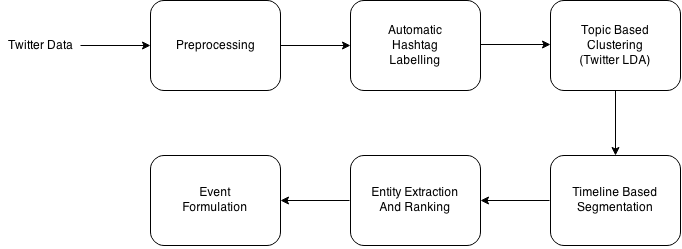
\includegraphics[width=0.8\textwidth]{Detection1.png} 
    \caption{Event Detection Pipeline} 
    \label{fig:pipeline}
\end{figure*}

Fig. \ref{fig:pipeline} shows the complete pipeline of our event detection system. The first and foremost step is to pre-process Twitter data. This step is of paramount importance because Twitter data is extremely noisy and contains a lot of irrelevant and redundant information that have are either not informative and interesting or have no bearing on event extraction process. The processed Twitter data is then fed into the event extraction pipeline. One of the most important feature of Tweets for the purpose of event extraction is hashtag. Hashtags generally suggestive of the context of the Tweet. Albeit noisy, hashtags attempt to capture the situation, event, or incident which the tweet talks about and is representative of the context embedded in the tweet. However, only a small fraction of tweets are hashtagged by the users. This calls for automatic hashtag recommendation for untagged tweets. The hashtags are of prime importance to the Twitter LDA used in the Topic based Clustering module. It segregates the tweets into topic clusters where each cluster could potentially represent a general topic like bomb-blast or election. This is followed by timeline based segmentation of tweets in each topic cluster. To pin-point specific event instances, named entity recognition is employed to extract entity mentions in the tweets. Finally, event instances are formulated by combining the topic, timeline, and entity information extracted from the pipeline. The structure of the pipeline imparts an inherent hierarchy in the event extraction process.

In the following sections, we discuss each module separately in detail, describing the technical details involved.

\section{Pre-Processing}
The pre-processing step involves cleaning the Twitter data to get rid of noise elements. In particular, HTML tags, URLs, \@user mentions, re-tweets, and hashtags are removed. Next, stop words that occur very frequently such as \textit{a, the, that, etc.} are removed because they are not informative. Additionally, an online slang dictionary \footnote{\url{http://www.noslang.com/dictionary/}} is used to convert Internet slang into their corresponding English words. This step is very important because Twitter posts are full of misspelled and slang words because of the restriction on number of characters in a tweet. A comprehensive dictionary based slang conversion works reasonably well because significant portion of the Internet slang is standardized - \textit{u} for you; \textit{2morrow, 2morow, tomorow} for tomorrow; \textit{bcoz, coz, cz} for because.

\section{Automatic Hashtag Labelling}
As discussed above, hashtags capture the context of a tweet. They can be visualized as annotations given by humans to each tweet. Hence, they could, to some extent, be used to capture topics embedded in tweets. Our Topic Extraction module relies on the abundance and reliability of these tagged tweets. While these tags are not a necessity, the performance of the Topic Extraction process increases drastically if a significant number of tweets are hashtagged. However, as observed in \cite{mehrotra2013improving}, only about $22.3\%$ tweets are labelled; even among these, only $~19\%$ are specific.

To circumvent this deficiency of tagged tweets, we have used a simple tweet recommendation system. First, all the pre-hashtagged tweets are put together. Then untagged tweets are then scored against each tweet in the tagged tweet pool. The similarity measure used is cosine similarity based on TF and TF-IDF scores. If the similarity score of an untagged tweet and a tagged tweet exceeds a threshold $c$, then the hashtags of the tagged tweet are considered as potential candidates for the untagged tweet. Among all the potential candidates, the top $3-5$ candidates are assigned to the untagged tweet.

\section{Topic Extraction}
The first level in our hierarchical event extraction pipeline segregates tweets into topics. Each topic consists of a set of tweets that are related to each other. Each such cluster is intended to correspond to a broad topic such as \textit{bomb blast}, \textit{Hollywood}, \textit{technology}, etc. The intuition is to cluster the tweets into broad sets of related tweets. Each set could potentially contain numerous instances of events that might or might not be directly connected, but could be grouped superficially under the purview of their topic. This hierarchical approach facilitates the event evolution and tracking process. Attempting to zero down on specific event instances directly at first level could be computationally expensive (due to huge size of Twitter dataset and the Named-Entity extraction), as opposed to segregating tweets into smaller, related sets. Moreover, same entities could be involved in events which are completely unrelated to each other. For example, entity \textit{Guwahati} could occur in sporting event as well as movie screening. Without top level topic segmentation, the event evolution and tracking part might incorrectly fall into relating these two events. With high level topic segmentation, event tracking could be accomplished within the logical domain of a topic.

To this end, we employ Topic Modeling techniques like LDA which infer topic distributions in documents in an unsupervised manner. Applying LDA on Twitter data masqueraded as documents gives us logical clusters of related tweets with each clustering representing a topic. Traditional LDA works well on structured documents like news-wire data, articles, and blogs. Due to the noisy, sparse, extremely short, and unstructured nature of micro-blogs, standard LDA fails to infer topic distributions. Several variants have been proposed in literature for the topic inferences on micro-blogs. We have employed Twitter LDA \cite{zhao2011comparing} for topic based clustering of tweets.

\begin{figure*}
 \centering
 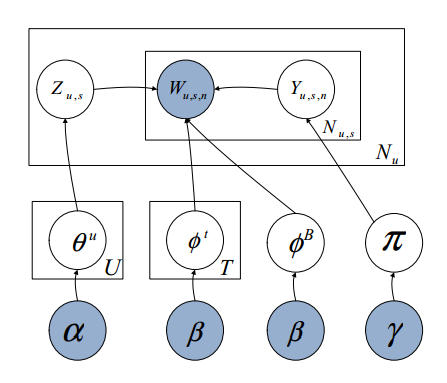
\includegraphics[width=0.5\textwidth]{twitter-lda}
 \caption{Twitter LDA Plate Notation}
 \label{fig:plate}
\end{figure*}

\subsection{Twitter LDA}{\label{sec:pipeline:tlda}}
An issue pertaining to the use of LDA on Twitter data is the questionable assumption of considering a tweet as a mixture of topics. Given the extremely short nature of tweets, most tweets consists of a single topic. Some studies have tackled this problem by aggregating the tweets of a user in a single document. This method, though effective, is not guaranteed to help much because of the fact that users generally express a wide variety of different topics in their tweets which may not be related to each other. This analysis will still be good if we want to profile users; but since our aim is to mine events from the topics, the possible solutions that seems feasible will be to aggregate tweets based on time, locality and hashtags.

To this end, \cite{zhao2011comparing} have proposed an effective variant of the standard LDA, called Twitter LDA. It is based on the assumption that a tweet will contain a single topic chosen from a topic distribution of a particular user. 

\paragraph{Model Description} 
The generative model makes the following assumptions. Twitter data has $T$ number of topics. When a user tweets, he/she selects a topic from his/her favorite list of topics, these topics will be from the T topics. Then for the selected topic, the user selects a bag of words, one by one from the distribution of words over topics. However, all the words of the tweet need not necessarily describe the topic. Many of them are just common words occurring in tweets of various different topics. So for each of the words, user first decides whether the given word is closely describes the topic or not. Depending upon this the word will be classified as a topic word or a background word. He then chooses the word from its respective distribution.

 \begin{figure*}
 \centering
 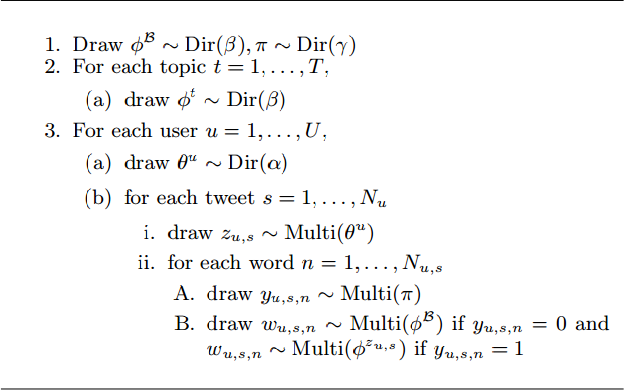
\includegraphics[width=0.6\textwidth]{lda-algo}
 \caption{Twitter LDA Generative Process}
 \label{fig:twitterlda-algo}
\end{figure*}

Formally, let $\theta_u$ denotes the topic distribution for a user $u$. Let $\phi_t$ be the distribution of words for the topic $t$ and let $\phi_B$ be the distribution of background words. $\pi$ is a Bernoulli distribution which denote the word belongs to the background class or to the topic class. $\alpha,~\beta,~\gamma$ are Dirichlet parameter used for generating respective Dirichlet distributions. The plate notation and generative algorithm are given in Fig.\ref{fig:plate} and Fig.\ref{fig:twitterlda-algo}.

We have used a variant of Twitter LDA for topic based clustering. Instead of aggregating tweets based on users, pooling tweets based on hashtags gives more coherent and logical topic clusters. Hashtag based tweet aggregation seems more intuitive because hashtags can be thought of as crude topic assignments manually given by users. Although LDA works in an unsupervised fashion, aggregating related tweets into a document could indirectly guide the inference process towards more sound topic clusters.

The Topic-based Clustering module was tested on the dataset using the tweaked version of Twitter LDA for different number of topics, such as $T=25$, $T=50$, and $T=100$. This segmented the tweets into clusters based on high level abstract topics. Each topic cluster could potentially contain numerous event instances. While high level topics correspond to the class of events, specific event instances are almost always associated with one or more entities such as location, person, organization etc. The next logical step would be, thus, to identify named entities in topic clusters to identify event instances. The Entity Extraction module deals with entity extraction and additional processing to pin-point event instances.

\section{Timeline based Segmentation}
Before proceeding to entity based segmentation, we segment each topic cluster based on timeline, creating sub-clusters within each topic corresponding to non-overlapping window lengths of $N$ days. Timeline based segmentation enables modeling of event evolution and temporal tracking.

\section{Entity Extraction and Ranking}
After getting the time segmented cluster of tweets, our aim is to find the important words, places, persons that will represent an event. For our purpose, we used the Twitter NER \cite{ritter2011named}. As noted in \cite{ritter2011named}, the reason behind using a NER specifically trained for twitter is that the tweets are generally noisy and that traditional NER tools do not work well for micro-texts. We have used the NER to extract the named entities and location information from the tweets. The named entities captured by Twitter NER includes persons, locations, organizations, movies etc. A subtlety to note is that the NER finds the location information from the text by using only the semantics of the text. To further increase the accuracy, we also pipelined NER with a dictionary based location detection mechanism which uses publicly available geo dictionary.

A significant number of tweets will not have any entity mentions. We can safely ignore these tweets because it is highly unlikely for a tweet to talk about an event without mentioning even a single event phrase or an associated entity.

\subsection{Entity-based Clustering}
Once we have extracted entities for each of the tweets, we proceed forward to make a entity set along with frequencies for each of the tweet sub-cluster (i.e. for each time-segment within each high-level topic). Tweets are grouped based on the entities present in them. At this second level, each tweet group comprises of tweets talking about a specific entity within a specific time segment under a high level topic. This level hence captures the high level topic, the temporal aspect, as well as the entity aspect of an event. On a superficial level, each tweet cluster at this level could potentially represent an event instance. However, there are numerous subtle fallacies in this approach, some of which are discussed and tackled below.

First, we rank each entity cluster using different scoring functions like frequency of occurrence and TD-IDF ranking. Only top $e$ tweet clusters (under the umbrella of a high-level topic, time segment, and an entity) are reported as event instances. Below, we discuss some of the observations of TF and TF-IDF ranking.

\paragraph{TF Ranking}
Each entity is scored by directly counting the number of tweets that mention that entity. Entities that have been more frequently mentioned are more likely to be involved in a trending event. Hence, focusing on most talked about entities works reasonably well for the purpose of detection. However, the analysis of our test runs on the dataset revealed a subtle flaw in this approach. Some common entities like Twitter, Facebook, Myspace, YouTube appeared among the top entities set in every topic. Manual cross-checking with the dataset revealed that it was indeed true that surprisingly large number of tweets mentioned these entities. While some tweets did indeed talk about an event related to these entities, most of them represented general personal experiences and musings of the users with these social platforms. These overly frequently entities are analogous to stop-words in a text. While, in principle, they could potentially be informative (and hence, represent an event instance), more often than not, they are associated with noise information.

\paragraph{TF-IDF Ranking}
One possible way to mitigate the issue of over-rewarding of the "stop-word entities" is to completely ignore these entities from our pipeline. However, this approach seems to pessimistic since occasionally these entities could indeed correspond to an event instance. A more optimistic way to circumvent this issue is to use TF-IDF ranking of entities, with TF being the number of tweets in a time segment mentioning the entity, and IDF being the inverse of the number of time-segments over all high-level topics in which this entity occurs. While this ranking handles the issue of "stop-word entities", it introduces other issues. Most of the entities that came at top were the ones with TF-IDF score 1, i.e. those that occurred only in a single time segment. This could be handled by ignoring entities present only in very few time segments. Once again, this is an approximation which could lead to discarding of many event instances. This is based on the assumption that it is highly unlikely that an event occurs which is talked about only during very few time periods and the number of tweet mentions drops down significantly outside those time frames. This could be ensured by meticulously choosing the length of a time segment and TF-IDF threshold.

\subsection{Merging Entities} \label{section:cooccurence}
Our abstraction of associating each entity based cluster at the second level to an event instance is primitive and flawed. It fails to capture the fact that an event instance could be associated to more than one entities. To this end, some post-processing is done on the entity sets to combine logically connected entities such as Apple and Ipad into a single entity. Without entity merging, we could incorrectly infer that the Apple cluster and the Ipad cluster correspond to two separate event instances. To this end, we propose entity merging schemes based on maximum common subsequence and co-occurrence frequencies. These are discussed below.

\paragraph{Maximum Common Subsequence}
First and foremost, we merge entities that indeed correspond to the same entity in the real world, but were extracted as separate ones because of common spelling variations or the entity being composed of two or more space separated words, with different users using different components of the entity words to refer to the entity. For example, entities like \textit{Bieber} and \textit{Justin Bieber} actually refer to the same person, but both of them are used to refer to him. Such entities could be merged by computing the maximum common subsequence (potentially dis-contiguous) between each pair of entities and merging those whose maximum common subsequence exceeds a threshold. Advantage of looking for common subsequence over common substring is that it handles spelling variations as well.

\paragraph{Direct co-occurrence frequency}
Co-occurrence of each pair of entity is computed within a high-level topic cluster by counting the number of tweets $t_k$ in which the two entities $e_i$ and $e_j$ co-occur using the following formula.

\begin{equation}
\frac{\sum_k\delta(e_i, t_k) \cdot \delta(e_j, t_k)}{K}
\end{equation}
	
where, $K$ is the total number of tweets in the high-level topic cluster, and 

% $\delta(e_i, t_k)~=~$
% \[ \begin{cases} 
%       $1$ & $e_i \in t_k$ \\
%       $0$ & otherwise 
%   \end{cases}
% \]

$$
\delta(e_i, t_k)~=~ = \left\{
        \begin{array}{ll}
            1 & e_i \in t_k \\
            0 & otherwise 
        \end{array}
    \right.
$$

Direct co-occurrence based merging does not give acceptable results because it is unlikely that a single tweet contains both the entities that we should be logically merged. This can attributed to the restriction on the length of each tweet as well as the general inclination towards brevity in micro-blogs as opposed to redundancy in larger articles. Hence, the co-occurrence scores are subdued.

\paragraph{Hashtag based co-occurrence}
As noted above, it is unlikely for two related entities to co-occur in a single tweet. However, in a set of tweets related to the two entities, the co-occurrence is expected to be high. In this method, instead of measuring co-occurrence at individual tweet level, we measure co-occurrence at the level of a group of related tweets for gauging the logical relation of two entities. This tackles the sparseness at the level of individual tweets by expanding the domain of search to a collection of tweets. 

Hashtags are exploited to construct the set of tweets related to a pair of entities. Since hashtags capture the context of a tweet, tweets with same hashtags are likely to be related, albeit on a potentially superficial level. Hashtags are noisy and the same hashtag could correspond to different situations. This problem could be mitigated to some extent by restricting the domain of search to the high-level topic cluster returned by Twitter LDA or to an even more restrictive time segmented cluster.

\section{Event Formulation}
Each entity cluster at the bottom level (after performing entity merging) represents an event instance. At this level, each cluster is associated with a high level topic (assigned by Twitter LDA) like \textit{bomb blast}, a time segment (due to timeline segmentation), and a set of entities (assigned by Twitter NER and entity merging). An event instance is formulated as an object having a number of attributes which include a set of entities, time frame, high-level topic, and a set of keywords describing an event. The set of keywords describing the event are extracted using Twitter NER, which has a special tag \textit{B-EVENT} for words describing an event. These words generally include verbs, adjectives, and adverbs like \textit{quitting}, \textit{death}, \textit{going up} etc.